\documentclass{standalone}

%----------------------------------------------------------------------------------------------%
%                                 Packages and basic declarations
%----------------------------------------------------------------------------------------------%

\usepackage{amsmath}
\usepackage{mathrsfs}
\usepackage{pgf}
\usepackage{tikz}
\usepackage{verbatim}

%\usetkzobj{all}
\usetikzlibrary{arrows}



%----------------------------------------------------------------------------------------------%
%----------------------------------------------------------------------------------------------%
%                                            DOCUMENT STARTS
%----------------------------------------------------------------------------------------------%
%----------------------------------------------------------------------------------------------%

\begin{document}

%----------------------------------------------------------------------------------------------%
%                Single RVE with applied constant strain, only debonded
%----------------------------------------------------------------------------------------------%
 
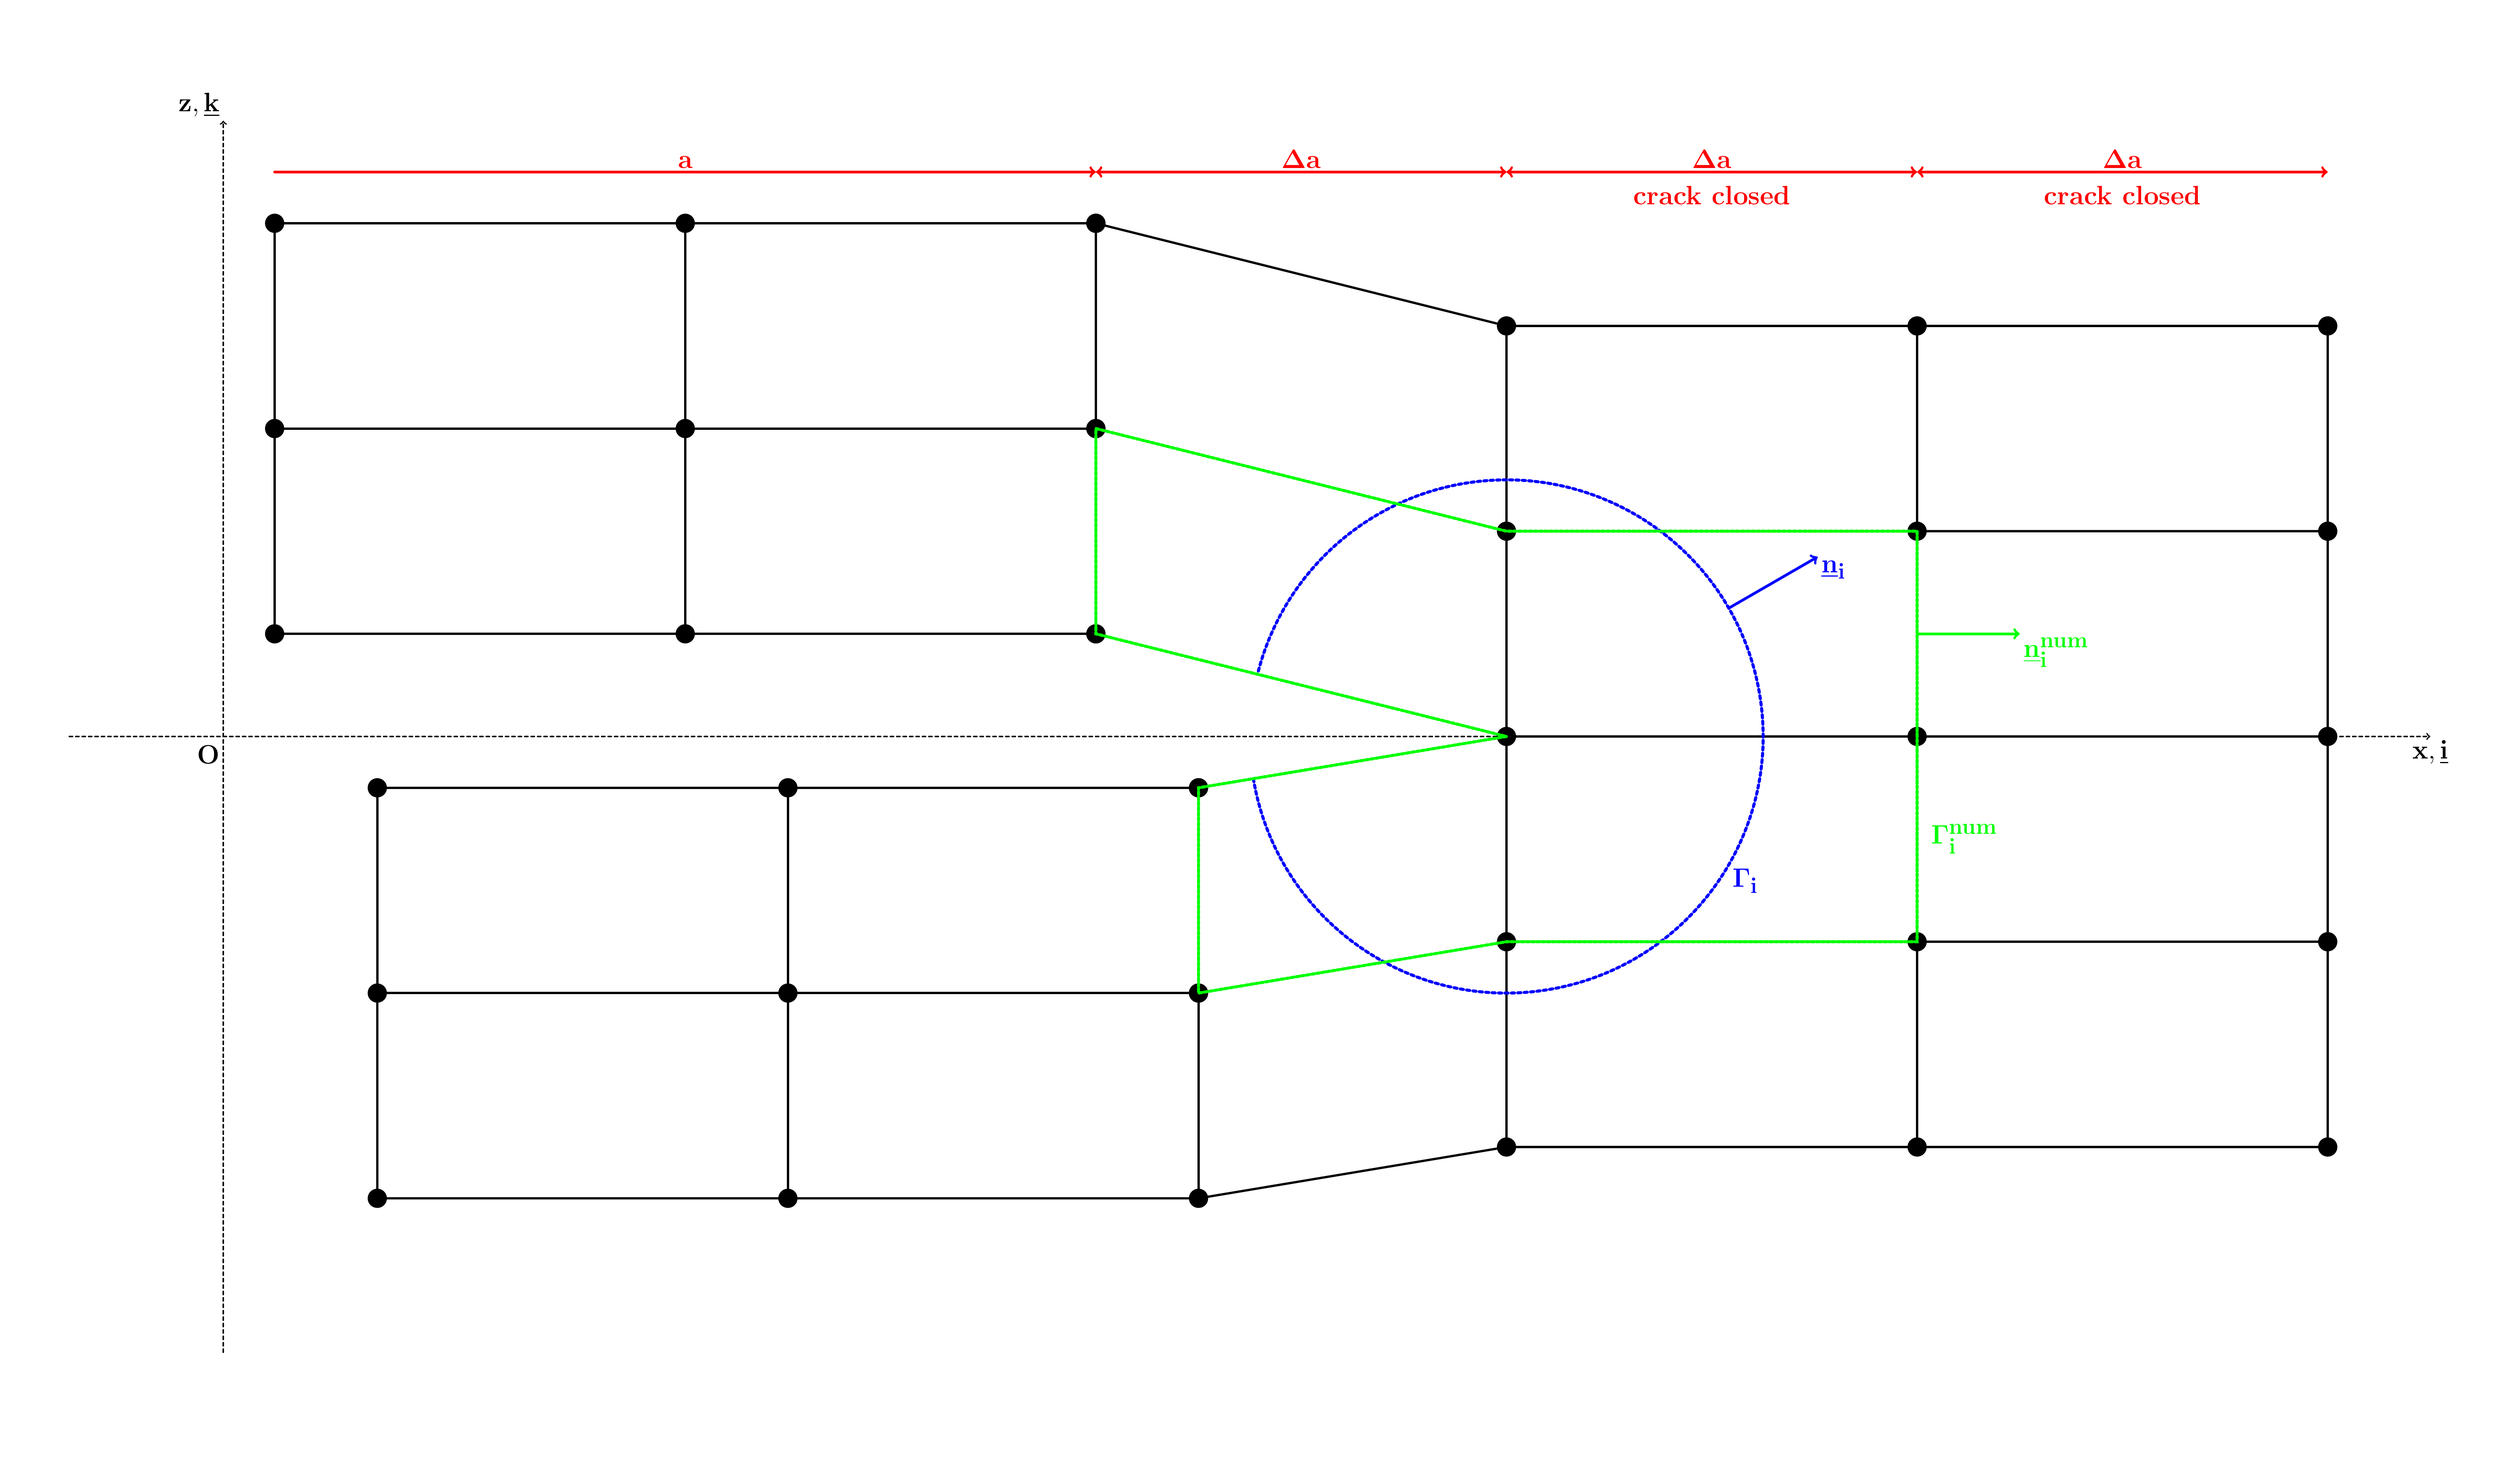
\begin{tikzpicture}[scale=4.5,cap=round,x=1.5cm,y=1.5cm]

%----------------------------------------------------------------------------------------------%
%                                                   CONSTANTS
%----------------------------------------------------------------------------------------------%

\def\pivalue{3.141592653589793238462643383279502884197169399375105820974944592307816406286}



\draw[->,dashed, line width = 0.5mm] (-7,0) -- (4.5,0);
\node[anchor=north] at (4.5,0) {\Huge $\mathbf{x,\underline{i}}$};
\draw[->,dashed, line width = 0.5mm] (-6.25,-3) -- (-6.25,3) ;
\node[anchor=south east] at (-6.25,3) {\Huge $\mathbf{z,\underline{k}}$};

\node[text=black,anchor=north east] at (-6.25,-0.025) {\Huge $\mathbf{O}$};

\draw[line width=0.75mm] (4,0) -- (4,1) -- (2,1) -- (0,1) -- (-2,1.5) -- (-2,0.5) -- (0,0) -- (2,0) -- (4,0);
\draw[line width=0.75mm] (4,1) -- (4,2) -- (2,2) -- (0,2) -- (-2,2.5) --  (-4,2.5) -- (-6,2.5) -- (-6,1.5);
\draw[line width=0.75mm] (2,2) -- (2,1);
\draw[line width=0.75mm] (0,2) -- (0,1);
\draw[line width=0.75mm] (-2,2.5) -- (-2,1.5);
\draw[line width=0.75mm] (-4,2.5) -- (-4,1.5);
\draw[line width=0.75mm] (4,0) -- (4,-1) -- (2,-1) -- (0,-1) -- (-1.5,-1.25) --  (-1.5,-0.25) -- (0,0);
\draw[line width=0.75mm] (4,1) -- (4,-1);
\draw[line width=0.75mm] (2,1) -- (2,-1); 
\draw[line width=0.75mm] (0,1) -- (0,-1);
\draw[line width=0.75mm] (-2,1.5) -- (-4,1.5) -- (-6,1.5) -- (-6,0.5) -- (-4,0.5) -- (-2,0.5);
\draw[line width=0.75mm] (-1.5,-1.25) -- (-3.5,-1.25) -- (-5.5,-1.25) -- (-5.5,-0.25) -- (-3.5,-0.25) -- (-1.5,-0.25);
\draw[line width=0.75mm] (4,-1) -- (4,-2) -- (2,-2) -- (0,-2) -- (-1.5,-2.25) --  (-3.5,-2.25) -- (-5.5,-2.25) -- (-5.5,-1.25);
\draw[line width=0.75mm] (2,-2) -- (2,-1);
\draw[line width=0.75mm] (0,-2) -- (0,-1);
\draw[line width=0.75mm] (-1.5,-2.25) -- (-1.5,-1.25);
\draw[line width=0.75mm] (-3.5,-2.25) -- (-3.5,-1.25);
\draw[line width=0.75mm] (-4,1.5) -- (-4,0.5);
\draw[line width=0.75mm] (-3.5,-1.25) -- (-3.5,-0.25);

\draw[<->,line width=0.9mm,draw=red] (0,2.75) -- (-2,2.75);
\node[anchor= south,text=red] at (-1,2.75) {\Huge $\mathbf{\Delta a}$};
\draw[->,line width=0.9mm,draw=red] (-6,2.75) -- (-2,2.75);
\node[anchor= south,text=red] at (-4,2.75) {\Huge $\mathbf{a}$};
\draw[<->,line width=0.9mm,draw=red] (0,2.75) -- (2,2.75);
\node[anchor= south,text=red] at (1,2.75) {\Huge $\mathbf{\Delta a}$};
\node[anchor= north,text=red] at (1,2.7) {\Huge \bf{crack closed}};
\draw[<->,line width=0.9mm,draw=red] (2,2.75) -- (4,2.75);
\node[anchor= south,text=red] at (3,2.75) {\Huge $\mathbf{\Delta a}$};
\node[anchor= north,text=red] at (3,2.7) {\Huge \bf{crack closed}};


\coordinate(A)at(-2,0.5);
\coordinate(B)at(0,0);
\coordinate(C)at(-1.5,-0.25);    
\coordinate(D)at(0,2);   

\pgfmathanglebetweenpoints{\pgfpointanchor{B}{center}}{\pgfpointanchor{A}{center}}
\edef\angleOne{\pgfmathresult}
\pgfmathanglebetweenpoints{\pgfpointanchor{B}{center}}{\pgfpointanchor{C}{center}}
\edef\angleTwo{\pgfmathresult}

\pgfmathsetmacro\startcos{cos(\angleTwo-360.0)}
\pgfmathsetmacro\startsin{sin(\angleTwo-360.0)}
\pgfmathsetmacro\normalcos{cos(30)}
\pgfmathsetmacro\normalsin{sin(30)}
\draw[draw=blue,dashed,line width=1mm] (1.25*\startcos,1.25*\startsin)arc(\angleTwo-360.0:\angleOne:1.25);
\draw[->,draw=blue,line width=0.9mm] (1.25*\normalcos,1.25*\normalsin) -- (1.75*\normalcos,1.75*\normalsin);
\node[text=blue,anchor=north west] at (1.75*\normalcos,1.75*\normalsin) {\Huge $\mathbf{\underline{n}_{i}}$};
\node[text=blue,anchor=north west] at (1.25*\normalcos,1.25*-\normalsin) {\Huge $\mathbf{\Gamma_{i}}$};

\foreach \Point in {(4,0) , (4,1) , (2,1) , (0,1) , (-2,1.5) , (-2,0.5) , (0,0) , (2,0),(4,-1) , (2,-1) , (0,-1) , (-1.5,-1.25) ,  (-1.5,-0.25),(-2,1.5) , (-4,1.5) , (-6,1.5) , (-6,0.5) , (-4,0.5) , (-2,0.5),(-1.5,-1.25) , (-3.5,-1.25) , (-5.5,-1.25) , (-5.5,-0.25) , (-3.5,-0.25) , (-1.5,-0.25),(4,2) , (2,2) , (0,2) , (-2,2.5) ,  (-2,2.5) , (-4,2.5) , (-6,2.5),(4,-2) , (2,-2) , (0,-2) , (-1.5,-2.25) ,  (-3.5,-2.25) , (-5.5,-2.25)}{
    \fill \Point  circle[radius=2pt];
}

\draw[draw=green,dotted,line width=1mm] (2,0) -- (2,1) -- (0,1) -- (-2,1.5) -- (-2,0.5) -- (0,0) --  (-1.5,-0.25) -- (-1.5,-1.25) -- (0,-1) -- (2,-1) -- (2,0);

\node[anchor= south,text=red] at (-1,3.5) {};
\node[anchor= north,text=red] at (-1.75,-3.5) {};
\node[anchor= east,text=red] at (-7.25,0) {};
\node[anchor= west,text=red] at (4.75,0) {};
\draw[->,draw=green,line width=0.9mm] (2,0.5) -- (2.5,0.5);
\node[text=green,anchor=north west] at (2.5,0.5) {\Huge $\mathbf{\underline{n}_{i}^{num}}$};
\node[text=green,anchor=west] at (2.05,-0.5) {\Huge $\mathbf{\Gamma_{i}^{num}}$};


\end{tikzpicture}

\end{document}